% Gabarit pandoc des corrigés publiés (brut et guidé). Contenu sans marque ni nom de site.
% Compilation : lualatex (latexmk -lualatex).
% Le Markdown reste la source unique : ne pas éditer ce fichier .tex à la main.
\documentclass[11pt,a4paper]{article}

% --- Moteur, polices (Latin Modern) et langue ---------------------------------
\usepackage{iftex}
\ifLuaTeX\else\errmessage{Ce document se compile avec lualatex}\fi
\usepackage{amsmath,amssymb,mathtools}
\usepackage{fontspec}
% mathrm=sym : \mathrm prend ses glyphes dans la police mathématique (ℓ, μ, Ω), comme KaTeX.
\usepackage[math-style=TeX,bold-style=TeX,mathrm=sym]{unicode-math}
% Repli pour les glyphes absents de Latin Modern (indices et exposants Unicode,
% flèches, filets des schémas en texte, symboles) : DejaVu, puis Latin Modern Math
% (ℓ, lettres mathématiques Unicode des légendes).
\directlua{
  luaotfload.add_fallback("repliTexte", {"DejaVuSerif:mode=harf;", "DejaVuSans:mode=harf;", "file:latinmodern-math.otf:mode=harf;"})
  luaotfload.add_fallback("repliMono", {"DejaVuSansMono:mode=harf;", "DejaVuSans:mode=harf;", "file:latinmodern-math.otf:mode=harf;"})
}
\setmainfont{Latin Modern Roman}[RawFeature={fallback=repliTexte}]
\setsansfont{Latin Modern Sans}[RawFeature={fallback=repliTexte}]
\setmonofont{Latin Modern Mono}[RawFeature={fallback=repliMono}]
\setmathfont{Latin Modern Math}
\usepackage[french]{babel}
\frenchsetup{SmallCapsFigTabCaptions=false}

% --- Mise en page --------------------------------------------------------------
\usepackage[a4paper,margin=2.2cm,headheight=14pt,footskip=1.2cm]{geometry}
\usepackage{microtype}
\setlength{\emergencystretch}{4em}
\tolerance=1500
\setlength{\parindent}{0pt}
\setlength{\parskip}{0.55\baselineskip plus 2pt minus 1pt}
\usepackage{xcolor}
% Gris nommés : babel-french rend « ! » actif dans le document.
\definecolor{gris2}{gray}{0.98}
\definecolor{gris3}{gray}{0.97}
\definecolor{gris5}{gray}{0.95}
\definecolor{gris35}{gray}{0.65}
\definecolor{gris40}{gray}{0.60}
\definecolor{gris45}{gray}{0.55}
\definecolor{gris50}{gray}{0.50}
\definecolor{gris55}{gray}{0.45}
\definecolor{gris60}{gray}{0.40}
\definecolor{gris65}{gray}{0.35}
\definecolor{gris70}{gray}{0.30}
\definecolor{gris80}{gray}{0.20}
\definecolor{gris85}{gray}{0.15}
\usepackage{graphicx}
\usepackage{float}
\usepackage{caption}
\captionsetup{font=small,labelformat=empty,justification=centering}
\usepackage{booktabs,longtable,array,multirow,calc}
\usepackage{siunitx}
\sisetup{locale=FR}
\usepackage[version=4]{mhchem}
\usepackage{listings}
\usepackage{fancyhdr}
\usepackage{lastpage}
\usepackage[most]{tcolorbox}
\usepackage{enumitem}
\setlist{nosep,leftmargin=*,topsep=2pt}
\usepackage[hidelinks,unicode]{hyperref}
\usepackage{bookmark}
\hypersetup{pdftitle={Mines-Ponts MP — Chimie 2026 · Corrigé},pdfauthor={Rédigé par IA},pdfcreator={LaTeX},pdfsubject={Corrigé brut}}
\usepackage{xurl}

% --- Pandoc : listes, tableaux, figures ----------------------------------------
\providecommand{\passthrough}[1]{#1}
\providecommand{\tightlist}{\setlength{\itemsep}{0pt}\setlength{\parskip}{0pt}}

\makeatletter
\def\maxwidth{\ifdim\Gin@nat@width>\linewidth\linewidth\else\Gin@nat@width\fi}
\def\maxheight{\ifdim\Gin@nat@height>0.55\textheight 0.55\textheight\else\Gin@nat@height\fi}
\makeatother
\setkeys{Gin}{width=\maxwidth,height=\maxheight,keepaspectratio}
\setcounter{secnumdepth}{-\maxdimen}
\providecommand{\pandocbounded}[1]{#1}
\usepackage{longtable,booktabs,array}

% --- Code (listings) -----------------------------------------------------------
\lstset{
  basicstyle=\ttfamily\small,
  columns=fullflexible,
  keepspaces=true,
  breaklines=true,
  breakatwhitespace=false,
  postbreak=\mbox{\textcolor{gris50}{$\hookrightarrow$}\space},
  frame=single,
  rulecolor=\color{gris35},
  framesep=4pt,
  xleftmargin=5pt,xrightmargin=5pt,
  backgroundcolor=\color{gris3},
  keywordstyle=\bfseries,
  commentstyle=\color{gris65},
  stringstyle=\color{gris80},
  showstringspaces=false,
  tabsize=4,
  extendedchars=true,
  aboveskip=6pt,belowskip=6pt,
}

% --- Macros des corrigés (KaTeX ↔ LaTeX) ---------------------------------------
% Les corrigés sont écrits pour KaTeX : on définit ici ce que KaTeX connaît et
% que LaTeX n'a pas, sans jamais retoucher le Markdown.
\providecommand{\R}{\mathbb{R}}
\providecommand{\N}{\mathbb{N}}
\providecommand{\Z}{\mathbb{Z}}
\providecommand{\Q}{\mathbb{Q}}
\providecommand{\C}{\mathbb{C}}
\providecommand{\dd}{\mathrm{d}}
\providecommand{\llbracket}{\lBrack}
\providecommand{\rrbracket}{\rBrack}
\providecommand{\lBrace}{\lbrace}
\providecommand{\rBrace}{\rbrace}
\providecommand{\Box}{\square}
\providecommand{\Diamond}{\lozenge}
\providecommand{\varnothing}{\emptyset}
\providecommand{\argmax}{\operatorname*{arg\,max}}
\providecommand{\argmin}{\operatorname*{arg\,min}}
\renewcommand{\leq}{\leqslant}
\renewcommand{\geq}{\geqslant}

% Équation hors texte : réduite à la largeur de la ligne si elle déborde.
\newsavebox{\boiteequation}
\newcommand{\equationajustee}[1]{%
  \sbox{\boiteequation}{$\displaystyle #1$}%
  \ifdim\wd\boiteequation>\linewidth
    \[\resizebox{\linewidth}{!}{\usebox{\boiteequation}}\]%
  \else
    \[#1\]%
  \fi}

% --- Encadrés pédagogiques (sobres, lisibles en noir et blanc) -----------------
\tcbset{
  encadre/.style={
    enhanced,breakable,sharp corners,
    colback=white,colframe=gris55,
    boxrule=0.4pt,leftrule=2.2pt,
    left=6pt,right=6pt,top=3pt,bottom=3pt,
    before skip=6pt,after skip=6pt,
    fonttitle=\bfseries\small,coltitle=black,
    attach title to upper,after title={\quad},
    parbox=false,
  }
}
\newtcolorbox{indication}[1]{encadre,colframe=gris45,colback=gris2,title={Indication~#1}}
\newtcolorbox{methode}{encadre,colframe=gris70,title={Méthode}}
\newtcolorbox{piege}{encadre,colframe=gris85,boxrule=0.8pt,leftrule=2.2pt,title={Piège}}
\newtcolorbox{jury}{encadre,colframe=gris60,colback=gris5,title={Jury}}
\newtcolorbox{encadrenote}{encadre,colframe=gris40}

% --- Titres de section ---------------------------------------------------------
\usepackage{titlesec}
\titleformat{\section}{\Large\bfseries}{}{0pt}{}
\titleformat{\subsection}{\large\bfseries}{}{0pt}{}
\titleformat{\subsubsection}{\normalsize\bfseries}{}{0pt}{}
\titlespacing*{\section}{0pt}{14pt plus 4pt minus 2pt}{6pt}
\titlespacing*{\subsection}{0pt}{10pt plus 3pt minus 2pt}{4pt}
\titlespacing*{\subsubsection}{0pt}{8pt plus 2pt minus 2pt}{2pt}

% --- En-tête et pied de page ---------------------------------------------------
\pagestyle{fancy}
\fancyhf{}
\fancyhead[L]{\small\textsc{Corrigé brut} · Mines-Ponts MP}
\fancyhead[R]{\small Chimie 2026}
\fancyfoot[L]{\footnotesize Corrigé rédigé par IA, non officiel}
\fancyfoot[R]{\footnotesize \thepage\,/\,\pageref*{LastPage}}
\renewcommand{\headrulewidth}{0.4pt}
\renewcommand{\footrulewidth}{0pt}
\fancypagestyle{plain}{\fancyhf{}\fancyfoot[R]{\footnotesize \thepage\,/\,\pageref*{LastPage}}\fancyfoot[L]{\footnotesize Corrigé rédigé par IA, non officiel}\renewcommand{\headrulewidth}{0pt}}

\begin{document}
\thispagestyle{plain}
\begin{center}
  {\small\scshape Corrigé brut}\par\smallskip
  {\LARGE\bfseries Mines-Ponts MP — Chimie 2026 · Corrigé\par}\medskip
  {\large Mines-Ponts · MP · Chimie · 2026\par}
\end{center}
\vspace{2pt}\hrule\vspace{8pt}

\emph{Corrigé rédigé par IA, non officiel. Signalez toute erreur.}

Épreuve de 1 h 30, calculatrice interdite. « La chimie et le traitement des eaux » : 26 questions en deux parties indépendantes.

Les applications numériques utilisent les approximations de l'annexe 1 :

\begin{itemize}
\tightlist
\item
  \(\sqrt2\approx10/7\approx1{,}4\) et \(\ln10\approx2{,}3\) ;
\item
  \(\frac{RT}{\mathcal F}\ln x\approx0{,}06\log x\) (en V, à 298 K) ;
\item
  \(R\approx8\ \mathrm{J\cdot K^{-1}\cdot mol^{-1}}\) et \(\mathcal N_A\approx6\cdot10^{23}\ \mathrm{mol^{-1}}\).
\end{itemize}

Dans les quotients, les concentrations sont rapportées à \(c^\circ=1\ \mathrm{mol\cdot L^{-1}}\) et les pressions à \(P^\circ=1\) bar.

\hypertarget{traitement-des-eaux-par-le-procuxe9duxe9-uxe9lectro-fenton}{%
\section{Traitement des eaux par le procédé électro-Fenton}\label{traitement-des-eaux-par-le-procuxe9duxe9-uxe9lectro-fenton}}

\hypertarget{q1}{%
\subsection{Q1}\label{q1}}

Demi-équations des deux couples, avec leurs potentiels standard (annexe 3) :

\equationajustee{\begin{aligned}{}&\mathrm{HO^\bullet + H^+ + e^- = H_2O}, && E^\circ(\mathrm{HO^\bullet/H_2O})=2{,}80\ \mathrm V\\
&\mathrm{Cl_2 + 2\,e^- = 2\,Cl^-}, && E^\circ(\mathrm{Cl_2/Cl^-})=1{,}36\ \mathrm V
\end{aligned}}

L'oxydant le plus fort est celui du couple de potentiel standard le plus élevé. Comme \(2{,}80\ \mathrm V>1{,}36\ \mathrm V\) :

\textbf{Le radical hydroxyle \(\mathrm{HO^\bullet}\) est un oxydant plus fort que le dichlore.}

\hypertarget{q2}{%
\subsection{Q2}\label{q2}}

L'anode est l'électrode siège d'une oxydation, la cathode celle d'une réduction.

\begin{itemize}
\tightlist
\item
  Électrode A : \(\mathrm{H_2O} \longrightarrow \mathrm{\tfrac12\,O_2} + \mathrm{2\,H^+} + \mathrm{2\,e^-}\) ; l'eau perd des électrons, c'est une oxydation.
\item
  Électrode B : \(\mathrm{O_2} + \mathrm{2\,H^+} + \mathrm{2\,e^-} \longrightarrow \mathrm{H_2O_2}\) et \(\mathrm{Fe^{3+}} + \mathrm{e^-} \longrightarrow \mathrm{Fe^{2+}}\) ; ce sont des réductions.
\end{itemize}

\textbf{A est l'anode, B est la cathode.}

\hypertarget{q3}{%
\subsection{Q3}\label{q3}}

L'électrolyse est une transformation forcée : on relie la \textbf{plaque de graphite (anode)} au \textbf{pôle \(+\)} du générateur et le \textbf{feutre de carbone (cathode)} au \textbf{pôle \(-\)}. L'\textbf{ampèremètre} est branché \textbf{en série} dans le circuit extérieur (par exemple entre le pôle \(+\) et l'anode), sa borne d'entrée (mA) du côté du pôle \(+\).

\begin{figure}[H]
\centering
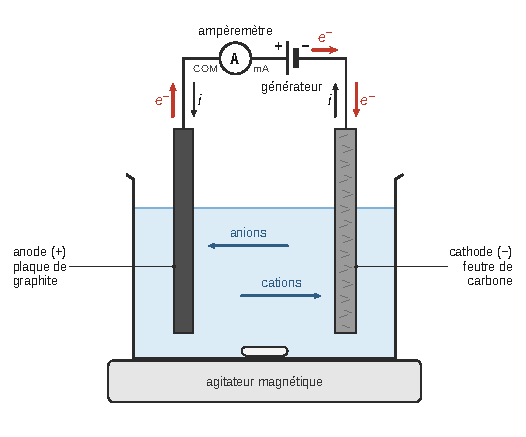
\includegraphics{figures/q3-dispositif-electro-fenton.pdf}
\caption*{Figure 1 --- Dispositif électro-Fenton complété : anode au pôle +,
cathode au pôle −, ampèremètre en série, électrons dans les fils
seulement}
\end{figure}

Sens des électrons : ils sont libérés à l'anode par l'oxydation, parcourent le fil de l'anode vers le pôle \(+\), traversent le générateur et partent du pôle \(-\) vers la cathode, où ils sont consommés par la réduction.

\textbf{Dans les fils, les électrons vont de l'anode vers la cathode (en passant par le générateur), en sens inverse du courant \(i\).} Dans la solution il n'y a pas d'électrons libres : le courant est porté par les ions (cations vers la cathode, anions vers l'anode).

\hypertarget{q4}{%
\subsection{Q4}\label{q4}}

On utilise un \textbf{montage à trois électrodes} :

\begin{itemize}
\tightlist
\item
  l'\textbf{électrode de travail} (carbone/graphite), siège des réactions étudiées, dont on fait varier le potentiel \(E\) ;
\item
  l'\textbf{électrode de référence} (électrode au calomel saturé, ou au chlorure d'argent), de potentiel connu et fixe, traversée par un courant nul ;
\item
  la \textbf{contre-électrode} (électrode auxiliaire, par exemple en platine), qui ferme le circuit.
\end{itemize}

\begin{figure}[H]
\centering
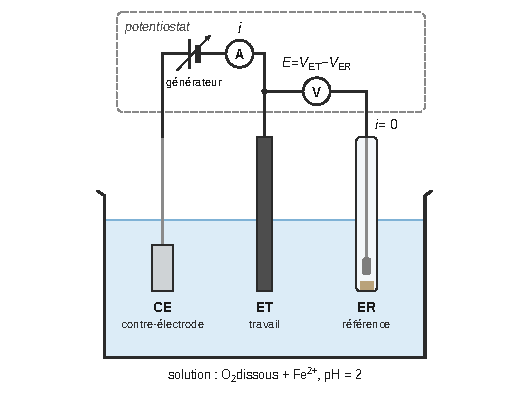
\includegraphics{figures/q4-montage-trois-electrodes.pdf}
\caption*{Figure 2 --- Montage à trois électrodes : i mesuré entre ET et CE, E
mesuré entre ET et ER}
\end{figure}

Branchements :

\begin{itemize}
\tightlist
\item
  un \textbf{générateur} de tension réglable (potentiostat) est relié entre l'électrode de travail et la contre-électrode ;
\item
  l'\textbf{ampèremètre} est \textbf{en série} dans ce circuit ET--CE et mesure \(i\) ;
\item
  le \textbf{voltmètre} est branché \textbf{entre l'électrode de travail et l'électrode de référence} et mesure \(E=V_{\mathrm{ET}}-V_{\mathrm{ER}}\).
\end{itemize}

On relève \(i\) en fonction de \(E\), avec \(i>0\) pour une oxydation.

\hypertarget{q5}{%
\subsection{Q5}\label{q5}}

Espèces présentes : \(\mathrm{H_2O}\), \(\mathrm{H^+}\) (pH 2), \(\mathrm{O_2}\) dissous, \(\mathrm{Fe^{2+}}\) ; pas de \(\mathrm{Fe^{3+}}\) initialement.

Les systèmes \(\mathrm{O_2/H_2O_2}\) (réduction) et \(\mathrm{O_2/H_2O}\) (oxydation) sont lents : leurs vagues sont décalées de \(-0{,}5\) V et \(+0{,}5\) V par rapport à leurs potentiels d'équilibre. Le système \(\mathrm{Fe^{3+}/Fe^{2+}}\) est rapide.

Un courant positif correspond à une oxydation, un courant négatif à une réduction. Description de la courbe, dans le sens des potentiels croissants :

\begin{longtable}[]{@{}
  >{\raggedright\arraybackslash}p{(\columnwidth - 2\tabcolsep) * \real{0.5016}}
  >{\raggedright\arraybackslash}p{(\columnwidth - 2\tabcolsep) * \real{0.4684}}@{}}
\toprule\noalign{}
\begin{minipage}[b]{\linewidth}\raggedright
Portion de la courbe
\end{minipage} & \begin{minipage}[b]{\linewidth}\raggedright
Réaction
\end{minipage} \\
\midrule\noalign{}
\endhead
\bottomrule\noalign{}
\endlastfoot
Branche cathodique raide, sans palier, aux potentiels les plus bas (mur du solvant) & \(\mathrm{2\,H^+} + \mathrm{2\,e^-} \longrightarrow \mathrm{H_{2(g)}}\) (réduction du solvant) \\
Vague cathodique avec palier de diffusion (potentiel voisin de \(0{,}69-0{,}06\times2-0{,}5\approx0{,}1\) V) & \(\mathrm{O_{2(aq)}} + \mathrm{2\,H^+} + \mathrm{2\,e^-} \longrightarrow \mathrm{H_2O_{2(aq)}}\) \\
Zone de courant nul & aucune réaction \\
Vague anodique raide avec palier de diffusion, démarrant vers \(0{,}68\) V (système rapide) & \(\mathrm{Fe^{2+}} \longrightarrow \mathrm{Fe^{3+}} + \mathrm{e^-}\) \\
Branche anodique raide, sans palier, aux potentiels les plus élevés (vers \(1{,}23-0{,}12+0{,}5\approx1{,}6\) V ; mur du solvant) & \(\mathrm{2\,H_2O} \longrightarrow \mathrm{O_{2(g)}} + \mathrm{4\,H^+} + \mathrm{4\,e^-}\) (oxydation du solvant) \\
\end{longtable}

\begin{figure}[H]
\centering
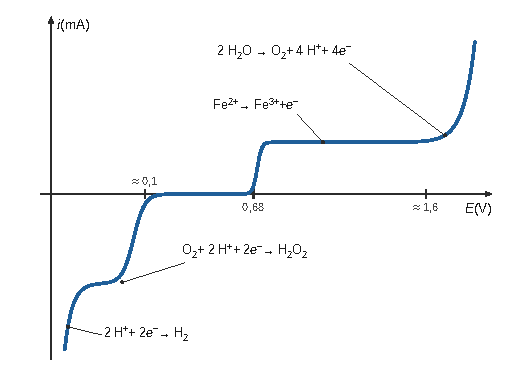
\includegraphics{figures/q5-courbe-intensite-potentiel.pdf}
\caption*{Figure 3 --- Courbe intensité-potentiel et réaction associée à chaque
portion}
\end{figure}

Les paliers correspondent à des espèces minoritaires (\(\mathrm{O_2}\) dissous, \(\mathrm{Fe^{2+}}\)) dont le courant est limité par la diffusion. Les branches extrêmes correspondent au solvant, en excès, sans palier. Le couple du fer n'a pas de branche cathodique, faute de \(\mathrm{Fe^{3+}}\).

\hypertarget{q6}{%
\subsection{Q6}\label{q6}}

La tension minimale est l'écart entre les potentiels auxquels démarrent les deux réactions voulues, surpotentiels compris.

\begin{itemize}
\tightlist
\item
  Cathode, \(\mathrm{O_2} + \mathrm{2\,H^+} + \mathrm{2\,e^-} \to \mathrm{H_2O_2}\) : \(E_c\approx E_{\mathrm{eq}}(\mathrm{O_2/H_2O_2})-0{,}5\) V.
\item
  Anode, \(\mathrm{2\,H_2O} \to \mathrm{O_2} + \mathrm{4\,H^+} + \mathrm{4\,e^-}\) : \(E_a\approx E_{\mathrm{eq}}(\mathrm{O_2/H_2O})+0{,}5\) V.
\end{itemize}

Les deux potentiels d'équilibre contiennent le même terme \(-0{,}06\,\mathrm{pH}\) (un proton par électron dans les deux couples) et la même pression de \(\mathrm{O_2}\). En prenant les autres activités égales à 1 :

\equationajustee{\begin{aligned}
U_{\min}&=E_a-E_c\\
&\approx(1{,}23+0{,}5)-(0{,}69-0{,}5)\\
&\approx0{,}54+1{,}0
\end{aligned}}

\equationajustee{\boxed{U_{\min}\approx1{,}5\ \mathrm V}}

À pH 2, on a \(E_c\approx0{,}07\) V et \(E_a\approx1{,}61\) V : même écart. En fonctionnement, il faut y ajouter la chute ohmique dans la solution.

\hypertarget{q7}{%
\subsection{Q7}\label{q7}}

Pour un élément des blocs \(s\) et \(p\), le nombre d'électrons de valence se lit sur la colonne de la classification : il vaut le numéro de colonne pour les colonnes 1 et 2, et ce numéro diminué de 10 pour les colonnes 13 à 18.

\begin{itemize}
\tightlist
\item
  \textbf{N} (colonne 15) : \textbf{5 électrons de valence}.
\item
  \textbf{O} (colonne 16) : \textbf{6 électrons de valence}.
\item
  \textbf{S} (juste sous O, donc colonne 16) : \textbf{6 électrons de valence}.
\end{itemize}

\hypertarget{q8}{%
\subsection{Q8}\label{q8}}

\textbf{Ion sulfate \(\mathrm{SO_4^{2-}}\)} : \(6+4\times6+2=32\) électrons, soit 16 doublets. Le soufre est l'atome central, lié aux quatre oxygènes.

\begin{itemize}
\tightlist
\item
  Représentation usuelle (S hypervalent, charges formelles minimisées) : deux liaisons \(\mathrm{S{=}O}\), chaque O portant 2 doublets non liants ; deux liaisons \(\mathrm{S{-}O^-}\), chaque O portant 3 doublets non liants et la charge formelle \(-1\) ; aucun doublet non liant sur S.
\item
  Une forme à quatre liaisons simples respecte l'octet et est aussi acceptable : S porte \(+2\), chaque O porte \(-1\) et 3 doublets non liants.
\end{itemize}

\textbf{Ion ammonium \(\mathrm{NH_4^+}\)} : \(5+4-1=8\) électrons, 4 doublets, tous liants. N est lié à quatre H par des liaisons simples, sans doublet non liant, et porte la charge formelle \(+1\).

\textbf{Peroxyde d'hydrogène \(\mathrm{H_2O_2}\)} : \(2\times6+2\times1=14\) électrons, 7 doublets. Enchaînement \(\mathrm{H{-}O{-}O{-}H}\) (3 doublets liants), chaque O portant 2 doublets non liants ; aucune charge formelle.

\begin{figure}[H]
\centering
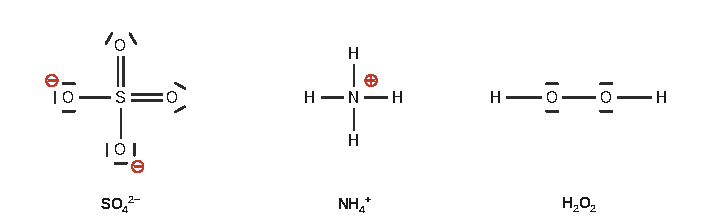
\includegraphics{figures/q8-schemas-lewis.pdf}
\caption*{Figure 4 --- Schémas de Lewis de l'ion sulfate, de l'ion ammonium et du
peroxyde d'hydrogène}
\end{figure}

\hypertarget{q9}{%
\subsection{Q9}\label{q9}}

Nombres d'oxydation du fer (O : \(-\mathrm{II}\), H : \(+\mathrm I\)) :

\begin{longtable}[]{@{}
  >{\raggedright\arraybackslash}p{(\columnwidth - 2\tabcolsep) * \real{0.5000}}
  >{\raggedright\arraybackslash}p{(\columnwidth - 2\tabcolsep) * \real{0.5000}}@{}}
\toprule\noalign{}
\begin{minipage}[b]{\linewidth}\raggedright
Espèce
\end{minipage} & \begin{minipage}[b]{\linewidth}\raggedright
n.o.(Fe)
\end{minipage} \\
\midrule\noalign{}
\endhead
\bottomrule\noalign{}
\endlastfoot
\(\mathrm{Fe_{(s)}}\) & \(0\) \\
\(\mathrm{Fe^{2+}}\) & \(+\mathrm{II}\) \\
\(\mathrm{Fe(OH)_{2(s)}}\) : \(x+2\times(-\mathrm I)=0\) & \(+\mathrm{II}\) \\
\(\mathrm{Fe^{3+}}\) & \(+\mathrm{III}\) \\
\(\mathrm{Fe(OH)_{3(s)}}\) : \(x+3\times(-\mathrm I)=0\) & \(+\mathrm{III}\) \\
\end{longtable}

\textbf{Classement vertical.} À pH fixé, le nombre d'oxydation croît avec le potentiel : le fer(III) est en haut, le fer(II) au milieu, le fer métallique (domaine E, sous la frontière horizontale la plus basse) en bas.

\textbf{Classement horizontal.} À nombre d'oxydation fixé, l'hydroxyde se forme par apport d'ions hydroxyde :

\equationajustee{\begin{aligned}{}&\mathrm{Fe^{3+}_{(aq)} + 3\,HO^-_{(aq)} = Fe(OH)_{3(s)}}\\
&\mathrm{Fe^{2+}_{(aq)} + 2\,HO^-_{(aq)} = Fe(OH)_{2(s)}}
\end{aligned}}

Il apparaît donc quand le pH augmente : l'ion libre occupe les pH acides, l'hydroxyde les pH plus élevés. D'où :

\equationajustee{\boxed{\begin{aligned}{}&\mathbf A:\ \mathrm{Fe^{3+}} && \mathbf B:\ \mathrm{Fe(OH)_{3(s)}}\\
&\mathbf C:\ \mathrm{Fe^{2+}} && \mathbf D:\ \mathrm{Fe(OH)_{2(s)}}\\
&\mathbf E:\ \mathrm{Fe_{(s)}}
\end{aligned}}}

Contrôles sur le diagramme :

\begin{itemize}
\tightlist
\item
  les frontières A/C et C/E sont horizontales (couples sans proton \(\mathrm{Fe^{3+}/Fe^{2+}}\) et \(\mathrm{Fe^{2+}/Fe}\)) ;
\item
  les frontières A/B (pH ≈ 1,7) et C/D (pH ≈ 7) sont verticales (précipitations) ; \(\mathrm{Fe(OH)_3}\) (\(\mathrm pK_s=38\)) précipite à pH beaucoup plus faible que \(\mathrm{Fe(OH)_2}\) (\(\mathrm pK_s=15\)) ;
\item
  la frontière B/C (\(\mathrm{Fe(OH)_3} + \mathrm{3\,H^+} + \mathrm{e^-} = \mathrm{Fe^{2+}} + \mathrm{3\,H_2O}\)) a une pente de \(-0{,}18\) V par unité de pH, trois fois plus forte que celles de B/D et D/E (\(-0{,}06\)).
\end{itemize}

\hypertarget{q10}{%
\subsection{Q10}\label{q10}}

Les ions \(\mathrm{Fe^{2+}}\) proviennent des 10 mL de solution de sel de Mohr :

\equationajustee{\begin{aligned}
n&=C_1V_1\\
&=4{,}5\cdot10^{-3}\times10\cdot10^{-3}\\
&=4{,}5\cdot10^{-5}\ \mathrm{mol}
\end{aligned}}

Le volume total vaut \(V=170+10=180\) mL (variation due au sulfate de sodium et aux gouttes d'acide négligée) :

\equationajustee{\begin{aligned}
C_0&=\frac{n}{V}\\
&=\frac{4{,}5\cdot10^{-5}}{0{,}180}
\end{aligned}}

\equationajustee{\boxed{C_0=2{,}5\cdot10^{-4}\ \mathrm{mol\cdot L^{-1}}}}

\hypertarget{q11}{%
\subsection{Q11}\label{q11}}

Équilibre de dissolution, écrit avec les ions hydroxyde :

\equationajustee{\mathrm{Fe(OH)_{3(s)} = Fe^{3+}_{(aq)} + 3\,HO^-_{(aq)}}}

Sa constante est \(K_s=[\mathrm{Fe^{3+}}][\mathrm{HO^-}]^3=10^{-38}\). Au début de la précipitation, le solide apparaît alors que tout le fer(III) est encore dissous : \([\mathrm{Fe^{3+}}]=C_0'\) et l'égalité \(C_0'[\mathrm{HO^-}]^3=K_s\) est vérifiée.

\equationajustee{\begin{aligned}
[\mathrm{HO^-}]^3&=\frac{10^{-38}}{10^{-4}}\\
&=10^{-34}\\
\mathrm{pOH}&=\frac{34}{3}\\
&\approx11{,}3
\end{aligned}}

\equationajustee{\boxed{\mathrm{pH}=14-11{,}3\approx2{,}7}}

L'expérience est menée à pH 2, inférieur à 2,7 : le fer(III) ne précipite pas. Il reste en solution et peut être réduit en fer(II) à la cathode, ce qui entretient le cycle catalytique de Fenton.

\textbf{C'est cohérent} : le pH 2 est choisi précisément pour éviter la précipitation de \(\mathrm{Fe(OH)_3}\), qui retirerait le fer du cycle. Avec \(C_0=2{,}5\cdot10^{-4}\) mol/L, la précipitation commencerait vers pH 2,5, toujours au-dessus de 2.

\hypertarget{q12}{%
\subsection{Q12}\label{q12}}

On règle le spectrophotomètre au \textbf{maximum d'absorption} du bleu de méthylène, lu sur l'annexe 6 :

\equationajustee{\boxed{\lambda\approx665\ \mathrm{nm}}}

À ce maximum, \(\varepsilon\) est le plus grand : la sensibilité de \(A\) à la concentration est meilleure. De plus \(\mathrm dA/\mathrm d\lambda=0\) : la mesure est peu sensible à une petite erreur de réglage de \(\lambda\).

Cette longueur d'onde est dans l'orange-rouge, couleur complémentaire du bleu : la solution paraît bleue parce qu'elle absorbe l'orange-rouge. Le bleu de méthylène étant la seule espèce colorée, l'absorbance ne mesure que lui.

\hypertarget{q13}{%
\subsection{Q13}\label{q13}}

Les produits étant incolores et l'absorbance proportionnelle à la concentration (loi de Beer-Lambert), \(A\) est proportionnelle à \([\mathrm{BM}]\). Le temps de demi-réaction est donc atteint quand l'absorbance est divisée par deux : \(A=A_0/2=0{,}937\).

Cette valeur est comprise entre \(A(240\ \mathrm s)=0{,}993\) et \(A(300\ \mathrm s)=0{,}863\). Interpolation linéaire :

\equationajustee{\begin{aligned}
t_{1/2}&\approx240+60\times\frac{0{,}993-0{,}937}{0{,}993-0{,}863}\\
&\approx240+26
\end{aligned}}

\equationajustee{\boxed{t_{1/2}\approx2{,}7\cdot10^2\ \mathrm s\ (\approx4{,}5\ \mathrm{min})}}

\hypertarget{q14}{%
\subsection{Q14}\label{q14}}

Pour une solution diluée d'une espèce absorbante de concentration \(c\), traversée sur une longueur \(\ell\) par une lumière monochromatique de longueur d'onde \(\lambda\) :

\equationajustee{A=\log\frac{I_0}{I}=\varepsilon(\lambda)\,\ell\,c}

\begin{itemize}
\tightlist
\item
  \(A\) : absorbance, sans dimension (\(I_0\) intensité incidente, \(I\) intensité transmise) ;
\item
  \(\varepsilon(\lambda)\) : coefficient d'absorption molaire, en \(\mathrm{L\cdot mol^{-1}\cdot cm^{-1}}\), dépendant de l'espèce, du solvant, de \(\lambda\) et de la température ;
\item
  \(\ell\) : longueur de solution traversée (largeur de la cuve), en cm ;
\item
  \(c\) : concentration de l'espèce absorbante, en \(\mathrm{mol\cdot L^{-1}}\).
\end{itemize}

Pour plusieurs espèces absorbantes, les absorbances s'ajoutent : \(A=\ell\sum_i\varepsilon_ic_i\). La loi est valable pour des solutions suffisamment diluées.

\hypertarget{q15}{%
\subsection{Q15}\label{q15}}

Loi de vitesse d'ordre 1, en réacteur fermé à volume constant. La vitesse de disparition du colorant est positive :

\equationajustee{v=-\frac{\mathrm d[\mathrm{BM}]}{\mathrm dt}=k[\mathrm{BM}]}

On sépare les variables et on intègre de \(0\) à \(t\) :

\equationajustee{\begin{aligned}
\frac{\mathrm d[\mathrm{BM}]}{[\mathrm{BM}]}&=-k\,\mathrm dt\\
[\mathrm{BM}](t)&=[\mathrm{BM}]_0\,e^{-kt}
\end{aligned}}

Le bleu de méthylène est la seule espèce colorée. Par la loi de Beer-Lambert à \(\lambda\) et \(\ell\) fixés, \(A(t)=\varepsilon\ell[\mathrm{BM}](t)\) et \(A_0=\varepsilon\ell[\mathrm{BM}]_0\), d'où \(A/A_0=[\mathrm{BM}]/[\mathrm{BM}]_0\) :

\equationajustee{\boxed{A(t)=A_0\,e^{-kt}}}

soit, de façon équivalente :

\equationajustee{\boxed{\ln A=\ln A_0-k\,t}}

(L'ordre 1 est un ordre apparent : la concentration en \(\mathrm{HO^\bullet}\), produit en continu, est supposée constante.)

\hypertarget{q16}{%
\subsection{Q16}\label{q16}}

D'après Q15, un ordre 1 impose que \(\ln A\) soit une fonction \textbf{affine} (et non linéaire : l'ordonnée à l'origine \(\ln A_0\) n'est pas nulle) décroissante de \(t\), de pente \(-k\).

Les points de la figure 5 sont bien répartis autour de la droite \(y=-2{,}23\cdot10^{-3}x+0{,}563\) (coefficient de corrélation, recalculé sur le tableau, \(r\approx-0{,}995\)). \textbf{L'allure est compatible avec un ordre 1}, avec toutefois une légère courbure systématique (points au-dessus de la droite aux extrémités, en dessous au milieu) qui montre que le modèle n'est qu'approché.

Par identification, la pente de la régression fournie vaut \(-k\) ; la constante de vitesse est positive :

\equationajustee{\boxed{k=2{,}23\cdot10^{-3}\ \mathrm{s^{-1}}}}

\hypertarget{q17}{%
\subsection{Q17}\label{q17}}

Éliminer 99 \% du colorant, c'est atteindre \([\mathrm{BM}]/[\mathrm{BM}]_0=A/A_0=10^{-2}\) :

\equationajustee{\begin{aligned}
e^{-kt_{99}}&=10^{-2}\\
t_{99}&=\frac{2\ln10}{k}\\
&=\frac{4{,}6}{2{,}23\cdot10^{-3}}
\end{aligned}}

\equationajustee{\boxed{t_{99}\approx2{,}1\cdot10^3\ \mathrm s\approx34\ \mathrm{min}}}

C'est bien plus que les 10 min de l'expérience, au bout desquelles il reste encore \(0{,}495/1{,}873\approx26\ \%\) du colorant.

\hypertarget{q18}{%
\subsection{Q18}\label{q18}}

Maille conventionnelle cubique à faces centrées : un cube d'arête \(a\), avec un atome à chacun des 8 sommets et au centre de chacune des 6 faces, et aucun atome au centre du cube.

\begin{figure}[H]
\centering
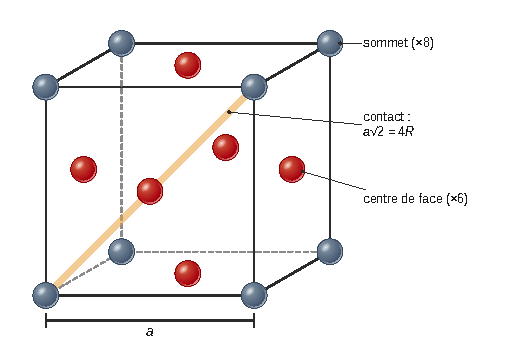
\includegraphics{figures/q18-maille-cfc.pdf}
\caption*{Figure 5 --- Maille cubique à faces centrées : 8 sommets, 6 centres de
faces, contact le long d'une diagonale de face}
\end{figure}

Population : chaque sommet est partagé entre 8 mailles, chaque centre de face entre 2 :

\equationajustee{\boxed{N=8\times\tfrac18+6\times\tfrac12=4\ \text{atomes par maille}}}

Coordinence (nombre de plus proches voisins d'un atome) : un atome de centre de face a pour plus proches voisins, à la distance \(a\sqrt2/2\), les 4 sommets de sa face et les 4 centres de faces de chacune des deux mailles qui partagent cette face (4 + 4 + 4) :

\equationajustee{\boxed{\text{coordinence }12}}

\hypertarget{q19}{%
\subsection{Q19}\label{q19}}

Les atomes sont tangents le long de la diagonale d'une face, de longueur \(a\sqrt2\), qui contient \(4R\) :

\equationajustee{\begin{aligned}
a\sqrt2&=4R\\
a&=2\sqrt2\,R\\
&\approx2\times\frac{10}{7}\times140\ \mathrm{pm}
\end{aligned}}

\equationajustee{\boxed{a\approx4{,}0\cdot10^2\ \mathrm{pm}=4{,}0\cdot10^{-10}\ \mathrm m}}

Avec \(\sqrt2\approx1{,}4\), on trouve \(a\approx392\) pm, même ordre de grandeur ; la valeur réelle pour le platine est 392 pm.

\hypertarget{q20}{%
\subsection{Q20}\label{q20}}

La masse volumique est la masse des atomes de la maille divisée par le volume \(a^3\) de la maille (cube) :

\equationajustee{\begin{aligned}
\rho&=\frac{N\,M(\mathrm{Pt})}{\mathcal N_A\,a^3}\\
&=\frac{4\times200\cdot10^{-3}}{6\cdot10^{23}\times(4{,}0\cdot10^{-10})^3}\\
&=\frac{0{,}8}{6\cdot10^{23}\times64\cdot10^{-30}}\\
&=\frac{0{,}8}{3{,}84\cdot10^{-5}}
\end{aligned}}

\equationajustee{\boxed{\rho\approx2{,}1\cdot10^4\ \mathrm{kg\cdot m^{-3}}\ (21\ \mathrm{g\cdot cm^{-3}})}}

Avec \(a=392\) pm, on trouve \(2{,}2\cdot10^4\ \mathrm{kg\cdot m^{-3}}\). La valeur réelle, 21,4 g/cm³, est bien retrouvée ; les écarts de quelques pour cent viennent des valeurs arrondies de \(M\) et \(\mathcal N_A\).

\hypertarget{traitement-des-eaux-par-des-procuxe9duxe9s-biologiques}{%
\section{Traitement des eaux par des procédés biologiques}\label{traitement-des-eaux-par-des-procuxe9duxe9s-biologiques}}

\hypertarget{traitement-des-eaux-en-milieu-auxe9robie}{%
\subsection{Traitement des eaux en milieu aérobie}\label{traitement-des-eaux-en-milieu-auxe9robie}}

\hypertarget{q21}{%
\subsection{Q21}\label{q21}}

Bilan en C (2 \(\mathrm{CO_2}\)), en H (3 \(\mathrm{H_2O}\)), puis en O (\(4+3=7=1+2\times3\)) :

\equationajustee{\boxed{\mathrm{C_2H_6O_{(aq)} + 3\,O_{2(aq)} \longrightarrow 2\,CO_{2(g)} + 3\,H_2O_{(\ell)}}}}

Contrôle électronique : le carbone passe de \(-\mathrm{II}\) (moyenne dans l'éthanol) à \(+\mathrm{IV}\), soit 12 électrons cédés, captés par 3 \(\mathrm{O_2}\) (\(3\times4=12\)).

\hypertarget{q22}{%
\subsection{Q22}\label{q22}}

Loi de Hess, avec les nombres stœchiométriques de Q21 :

\equationajustee{\begin{aligned}
\Delta_rH^\circ&=2(-400)+3(-300)-(-300)-3(-10)\\
&=-1370\ \mathrm{kJ\cdot mol^{-1}}
\end{aligned}}

\equationajustee{\begin{aligned}
\Delta_rS^\circ&=2(200)+3(50)-150-3(100)\\
&=+100\ \mathrm{J\cdot K^{-1}\cdot mol^{-1}}
\end{aligned}}

En convertissant \(\Delta_rS^\circ\) en \(\mathrm{kJ\cdot K^{-1}\cdot mol^{-1}}\) :

\equationajustee{\begin{aligned}
\Delta_rG^\circ&=\Delta_rH^\circ-T\Delta_rS^\circ\\
&=-1370-298\times0{,}100\\
&\approx-1400\ \mathrm{kJ\cdot mol^{-1}}
\end{aligned}}

\equationajustee{\boxed{\Delta_rG^\circ\approx-1{,}4\cdot10^3\ \mathrm{kJ\cdot mol^{-1}}}}

Constante d'équilibre (\(\Delta_rG^\circ\) en \(\mathrm{J\cdot mol^{-1}}\)), puis passage au logarithme décimal :

\equationajustee{\begin{aligned}
\ln K_1^\circ&=-\frac{\Delta_rG^\circ}{RT}\\
&\approx\frac{1{,}4\cdot10^6}{8\times298}\\
&\approx5{,}9\cdot10^2\\
\log K_1^\circ&=\frac{\ln K_1^\circ}{\ln10}\\
&\approx\frac{587}{2{,}3}\\
&\approx2{,}5\cdot10^2
\end{aligned}}

\equationajustee{\boxed{K_1^\circ\approx10^{255}}}

Seul l'ordre de grandeur de l'exposant a un sens avec les données arrondies.

\textbf{Conclusion} : \(K_1^\circ\gg10^4\), la réaction est totale (quantitative) ; l'oxydation de l'éthanol par le dioxygène est thermodynamiquement très favorable. Elle est pourtant lente à température ambiante : les bactéries jouent le rôle de catalyseurs (enzymes), elles accélèrent la réaction sans modifier \(K_1^\circ\).

\hypertarget{traitement-des-eaux-en-milieu-anauxe9robie-duxe9pourvu-doxyguxe8ne}{%
\subsection{Traitement des eaux en milieu anaérobie (dépourvu d'oxygène)}\label{traitement-des-eaux-en-milieu-anauxe9robie-duxe9pourvu-doxyguxe8ne}}

\hypertarget{q23}{%
\subsection{Q23}\label{q23}}

L'oxygène, plus électronégatif que l'azote, a le nombre d'oxydation \(-\mathrm{II}\). La somme des nombres d'oxydation est égale à la charge de l'ion :

\equationajustee{x+3(-\mathrm{II})=-\mathrm I}

\equationajustee{\boxed{\text{n.o.(N)}=+\mathrm V\ \text{dans}\ \mathrm{NO_3^-}}}

\hypertarget{q24}{%
\subsection{Q24}\label{q24}}

Équilibrage en N, puis O (par \(\mathrm{H_2O}\)), H (par \(\mathrm{H^+}\)), charges (par \(e^-\)). On vérifie que \(10=2\times5\) électrons correspondent au passage de N de \(+\mathrm V\) à \(0\) :

\equationajustee{\boxed{\mathrm{2\,NO^-_{3(aq)} + 12\,H^+_{(aq)} + 10\,e^- = N_{2(g)} + 6\,H_2O_{(\ell)}}}}

Formule de Nernst : l'oxydant et \(\mathrm{H^+}\) au numérateur, le diazote gazeux par sa pression partielle au dénominateur, l'eau solvant d'activité 1 :

\equationajustee{\boxed{E_1=1{,}25+\frac{0{,}06}{10}\log\left(\frac{[\mathrm{NO_3^-}]^2\,[\mathrm{H^+}]^{12}}{(c^\circ)^{14}}\cdot\frac{P^\circ}{P_{\mathrm{N_2}}}\right)}}

soit \(E_1=1{,}25+0{,}012\log\dfrac{[\mathrm{NO_3^-}]}{c^\circ}-0{,}072\,\mathrm{pH}-0{,}006\log\dfrac{P_{\mathrm{N_2}}}{P^\circ}\).

\hypertarget{q25}{%
\subsection{Q25}\label{q25}}

Le carbone passe de \(+\mathrm{IV}\) (\(\mathrm{CO_2}\)) à \(-\mathrm{II}\) (moyenne dans l'éthanol) : \(2\times6=12\) électrons.

\equationajustee{\boxed{\mathrm{2\,CO_{2(g)} + 12\,H^+_{(aq)} + 12\,e^- = C_2H_6O_{(aq)} + 3\,H_2O_{(\ell)}}}}

Le dioxyde de carbone, gazeux, intervient par sa pression partielle :

\equationajustee{\boxed{E_2=-0{,}33+\frac{0{,}06}{12}\log\left(\frac{(P_{\mathrm{CO_2}}/P^\circ)^2\,([\mathrm{H^+}]/c^\circ)^{12}}{[\mathrm{C_2H_6O}]/c^\circ}\right)}}

soit \(E_2=-0{,}33+0{,}010\log\dfrac{P_{\mathrm{CO_2}}}{P^\circ}-0{,}06\,\mathrm{pH}-0{,}005\log\dfrac{[\mathrm{C_2H_6O}]}{c^\circ}\).

\hypertarget{q26}{%
\subsection{Q26}\label{q26}}

L'oxydant le plus fort (\(\mathrm{NO_3^-}\), \(E^\circ=1{,}25\) V) réagit avec le réducteur le plus fort (\(\mathrm{C_2H_6O}\), \(E^\circ=-0{,}33\) V).

On combine \(6\times\)(Q24) et \(5\times\)(Q25 renversée), soit \(n=60\) électrons échangés. Après simplification de \(60\,\mathrm{H^+}\) et \(15\,\mathrm{H_2O}\) :

\equationajustee{\boxed{\mathrm{5\,C_2H_6O_{(aq)} + 12\,NO^-_{3(aq)} + 12\,H^+_{(aq)} \longrightarrow 10\,CO_{2(g)} + 6\,N_{2(g)} + 21\,H_2O_{(\ell)}}}}

(C : 10 = 10 ; N : 12 = 12 ; H : 42 = 42 ; O : 41 = 41 ; charges : 0 = 0.)

À l'équilibre, les potentiels des deux couples sont égaux ; en regroupant les termes logarithmiques de \(E_1=E_2\), on obtient :

\equationajustee{\begin{aligned}
\log K_2^\circ&=\frac{n\,\big(E^\circ(\mathrm{NO_3^-/N_2})-E^\circ(\mathrm{CO_2/C_2H_6O})\big)}{0{,}06}\\
&=\frac{60\times(1{,}25+0{,}33)}{0{,}06}\\
&=1580
\end{aligned}}

\equationajustee{\boxed{K_2^\circ=10^{1580}}}

(Si l'on écrit l'équation avec un nombre stœchiométrique 1 pour l'éthanol, \(n=12\) et \(K_2^\circ=10^{316}\).)

\textbf{Conclusion} : la constante est immense, la réaction est totale. L'oxydation de la matière organique par les nitrates est thermodynamiquement très favorable ; elle élimine à la fois la pollution organique et les nitrates, transformés en diazote gazeux. Comme en milieu aérobie, la réaction est lente et ce sont les bactéries qui la catalysent.

\end{document}
